\chapter{Importations et exportations de données}

\section{Présentation}

Le logiciel Filo-Science intègre deux modules génériques permettant de réaliser soit des importations, soit des exportations. 
Le premier vise à importer des données de pistage de poissons ou des données transmises par des sondes d'analyse physico-chimique. Les données fournies sont de type tabulé (fichiers ressemblant à des fichiers CSV).
Le second sert à générer un export de données au format JSON, pouvant comprendre également les informations rattachées, pour pouvoir les réimporter dans une autre base de données.

Les tables qui permettent de décrire ces fonctions sont stockées dans le schéma \textit{import} (figure \ref{fig:export_schema}).
\begin{figure}[h!]
\begin{center}
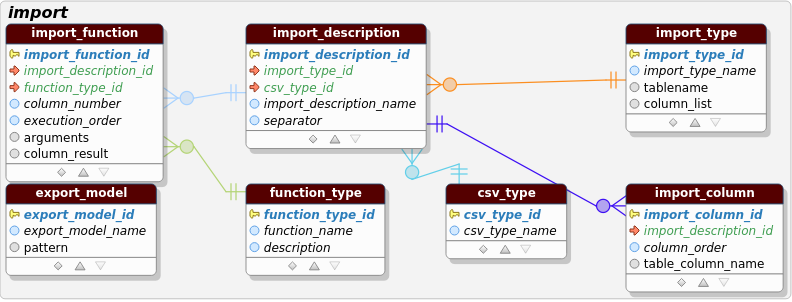
\includegraphics[width=\linewidth]{images/export_schema}
\captionof{figure}{Schéma des tables utilisées pour décrire les importations/exportations}
\label{fig:export_schema}
\end{center}
\end{figure}

\section{Importation de données tabulées}

Les structures des fichiers fournis par les systèmes d'acquisition automatique sont très variées, les données nécessitent souvent d'être reformatées ou recalculées avant de pouvoir être importées dans une table.

Le principe d'importation est le suivant :
\begin{itemize}
	\item chaque champ (une colonne) du fichier à importer peut faire l'objet d'une ou plusieurs transformations ou contrôles ;
	\item une fois l'ensemble de ces opérations réalisées, les champs pertinents vont être assignés à des colonnes de la table cible, et l'enregistrement réalisé en base de données.
\end{itemize}

\subsection{Types d'import}

Trois types d'import sont décrits et fournis, qui permettront d'alimenter les tables \textit{detection}, \textit{probe\_measure} et \textit{location}. 
La liste des colonnes utilisables pour l'importation est décrite, chaque colonne étant séparée par une virgule.

Les types d'import ne doivent pas être modifiés.

\subsection{Types de fonctions}

Les fonctions, codées dans l'application, sont décrites dans la table \textit{function\_type}. Cette table ne peut pas être modifiée.

Le tableau xx présente la liste des fonctions utilisables pour préparer un import.

% \usepackage{array} is required
\begin{tabular}{|c|>{\raggedright\arraybackslash}p{5cm}|c|c|}
\hline 
Nom de la fonction & Description & Contrôle ? & Transformation ? \\ 
\hline 
testValue & Teste si un champ contient la valeur indiquée & X &  \\ 
getSecondsFromTime & Transforme un champ de type hh:mm:ss.u en ss.u &  & X \\ 
extractRightChar & Extrait les n caractères à droite du champ &  & X \\ 
concatenateDateAndTime & Concatène un champ date et un champ time. L'argument doit correspondre au numéro de la colonne time &  & X \\ 
transformJulianToDate & Transforme un nombre de jours depuis la date indiquée en référence (au format Y-m-d) en date exploitable au format Y-m-d &  & X \\ 
verifyTypeNumber & Vérifie si une valeur est numérique ou non & X &  \\ 
testColumnsNumber & Vérifie que le nombre de colonnes de la ligne courante correspond bien au nombre attendu &  & X \\ 
getIndividualFromTag & Récupère l'identifiant du poisson à partir du tag (RFID) &  & X \\ 
getIndividualFromTransmitter & Récupère l'identifiant du poisson à partir du transmetteur (radio ou acoustique) &  & X \\ 
numericToHexa & Transforme une valeur numérique en valeur Hexa, si celle-ci ne l'est pas. La valeur Hexa doit comprendre au moins une lettre.  &  & X \\ 
concatenate & Associe le contenu de colonnes ou du texte. L'argument doit être au format JSON, sous la forme : [{"type":"col","val":4}, {type:"str","val":":"}] &  &  \\ 
matchingCode & Remplace la valeur courante par une autre valeur, définie dans un argument JSON au format : {"valueSearched":correspondingValue, "2ndvalue":corresp2}. Pour la recherche des paramètres de sonde, valueSearched doit correspondre au libellé utilisé par la sonde, et correspondingValue à la valeur de la clé dans la table des paramètres &  & X \\ 
formatDateTime & Transforme une datetime dans un format reconnu par la base de données, à partir du format indiqué. Exemple : d/m/Y H:i:s pour une date de type 13/01/2019 08:50:00. La liste des formats autorisés est disponible ici : \href{https://www.php.net/manual/fr/datetime.createfromformat.php}{https://www.php.net/manual/fr/datetime.createfromformat.php}&  & X \\ 
decodeAll & Transforme un jeu de caractère particulier en UTF-8. L'argument doit comprendre le jeu de caractère à transcoder, par exemple UTF-32 &  & X \\ 
transformDecimalSeparator & Transforme la virgule en point, pour les champs décimaux en français &  & X \\ 
\hline 
\end{tabular} 